\chapter{Simulating cognate histories}
After some general remarks on the place of simulation studies in computational historical linguistics as well as the in-silico approach to evaluation, this chapter presents the simulation model which I am using in parallel to the NorthEuraLex data to evaluate lexical flow inference methods.

Unlike more detailed existing simulation models like \cite{hochmuth_ea_2008}, which have components for explicitly generating and modifying phonetic strings and modeling the geographical spread of languages, my model limits itself to modeling contact in the form of transmitting discrete units, i.e.\ it models loanwords on the level of cognacy, without generating actual phonetic forms. This creates data different from what historical linguistics would apply to decide whether lexemes were inherited or borrowed, but the shape of the data is exactly what will be needed to evaluate lexical flow inference algorithms. 

\section{Simulation and in-silico evaluation}

\subsection{Advantages and shortcomings of simulation}
A simulation model is an algorithm which models the behavior of some real-world system, and uses randomness to generate output which is similar to the output of the real system. For instance, an adequate model of an economy should generate time series of measures such as interest rates, inflation, and unemployment which behave just as erratically as their real-world equivalents. An adequate model of tree growth should generate trunk shapes and branch structures which look just like the ones we can observe on real trees.

A very popular application of simulation models is as a way of testing assumptions about how the actual data can be explained. If our model generates data which are indistinguishable from our real data according to some relevant measure, we can take this as evidence that we have correctly understood and formalized an interesting aspect of the problem.

Within linguistics, this paradigm has previously mainly been applied to language competition. \cite{schulze_ea_2008} give an overview of different attempts to let a distribution of language sizes (by number of speakers) emanate from minimalistic models, with the goal of mirroring the observable distribution as closely as possible. Many of the more successful models are agent-based, modeling individual speakers which can choose to take over the language of neighboring speakers based on a prestige value, or just the dominant language in the neighborhood.

Combining previous models for explaining the distibution of language sizes, \cite{oliveira_ea_2008} arrive at a model which captures the observable distribution of language family sizes. While the final model given in the appendix of the paper is rather simple, the authors report that in additional experiments, adding more complexity to the models (e.g.\ by including the effects of war and similar historical contingencies) did not have any influence on the overall good fit with observed family sizes. I will take this as an indication that attempting to include such effects into my model is just as unlikely to lead to different behavior, allowing me to keep my own simulation simple as well.

Establishing knowledge about real-world systems on the basis of simple simulations is frequently criticized as too reductionistic, and spectacularly wrong predictions resulting from simulation models may have contributed to wide-spread scepticism towards modern economic theories. The practical and far less controversial advantage of simulation models is that they allow us to generate arbitrary amounts of data to test algorithms on. This in-silico evaluation allows us to compensate for insufficient amounts of actual test data, or as additional cross-validation of models developed on (and optimized for subsets of) actual data.

This is the paradigm in which \cite{embleton1986} already worked. Her simulation model represents an early attempt to adequately model the influence of borrowing between neighboring languages on cognate-based phylogenetic inference. The model is similar in spirit to the one I am presenting in this chapter, in that it operates on the level of individual cognate replacement events. Unlike my model, it assumes that the process of language split can be modeled by recursive subdivision of a two-dimensional area, precluding the possibility of geographical spread. Also, borrowing events are modeled as independent, i.e. for every new borrowing event sampled according to a global borrowing rate, a language picks one of the neighboring languages as the donor language at random, whereas the model I present in this chapter samples an additional level of contact channels in order to mirror the strong tendency for loans to occur in `packages' triggered by historical events. 

\cite{murawaki2015} presents another approach which explicitly simulates the transmission of lexical items by borrowing among neighboring language varieties, but does not have a phylogenetic component. The structures produced are thus very similar to my concept of contact flow networks. Based on the cognacy overlaps resulting from simulation on different network typologies, Murawaki then performs phylogenetic analysis, with the somewhat surprising result that the phylogenetic signal tends to look tree-like on tree-like spatial structures, even if inheritance is not modeled. This could indicate that the usually very good fit of tree models does not necessarily have to result from tree-like evolution, but that wave-like change can just as easily lead to tree-like signals in certain geographical configurations, which has interesting implications for the debate between family tree and wave models of language change.

Unlike the other models, the rather complex simulation model by \cite{hochmuth_ea_2008} generates phonetic data, to which the authors then apply modern standard tools for phylogenetic tree and network inference. While they find the amount of simulated lateral contact to have little impact on the performance of tree inference algorithms, the behavior of phylogenetic network algorithms is described as very erratic.

The main difficulty in using simulation models is that they are necessarily based on a set of assumptions about the nature of the data, which might not be true in reality. What if the way in which we generate data fails to capture an important case that occurs in real data, and is then not covered by the algorithm which we developed and tested on simulated data? To keep this problem under control, it is always best to evaluate a system both against simulated and real data. In the realm of causal inference, there has been a very strong tendency to develop the theory and algorithms either on very well-studied toy examples, or on massive amounts of simulated data. This makes it difficult to assess the performance of these methods on large real-world datasets, a problem that we are going to be faced with again when evaluating their potential for lexical flow inference.

\subsection{Principles of in-silico evaluation}
When assessing the performance of a heuristic algorithm (i.e.\ one without provable properties), the classical framework is to collect a set of gold-standard data, and to let the algorithm run on the data, comparing the output to the gold-standard using a useful definition of true and false positives and negatives, and then quantifying the performance in terms of precision and recall. Since gold-standard data are often difficult to acquire in large quantities (the last chapter provides a very good example of the efforts that may be required), the conclusions made from evaluating an algorithm on real data often rest on unstable grounds.

In the absence of a large enough amount of gold-standard data, one can use simulated data to get an impression of how the algorithm would perform on other data of the same shape. To get informative results, quite a bit of effort needs to be invested into developing a simulation model which is adequate for the purpose. The main requirements are that the model should not be overly complex in order to decrease the risk of overfitting the algorithm to certain (possibly hidden) properties of the gold-standard data. In a simulation model, it is always tempting to capture all aspects of the real data, but such an approach will often require many decisions to be made with inadequate backing in data or theory.

For instance, the actual linguistic history of a region is shaped by many historical events such as invasions, political ideas, technical innovations, and the shape of trade networks. A simulation model could try to emulate all of these phenomena in order to arrive at realistic simulated histories, and use these events to generate linguistic data. The problem is of course that such a model would require a very explicit (and formalized or at least quantitative) theory of political events, predictions about the conditions under which they will occur, and many other components which would quickly explode into separate research projects if we want to justify all of the myriad decisions which would be involved in designing such a model. Keeping the model complexity low, and the number of design decisions at a minimum, helps to avoid introducing too many unwarranted assumptions.

To configure the parameters even of a small model, it is good scientific practice to use structural features or at least statistics estimated from real data to increase (and quantify) the amount of realism. For instance, we might want to put data on historically observed unemployment rates into an economic model, to estimate how strong we expect oscillations in this measure to be in reality. For a simulation of language history, we will need to estimate (and inform the model) how often languages tend to split, and how intensively they can borrow from neighboring languages.

\section{Generating phylogenies}
A core component of any simulation model in computational historical linguistics (and also of some of the more advanced statistical methods) is a generative description of possible tree shapes. In statistical methods, these models are used to efficiently sample the space of possible trees in order to find good phylogenies. In in-silico evaluation, some part of the generated tree is removed from the input data for an algorithm which tries to reconstruct the missing information, and can then be evaluated against the truth.

Evolutionary models of species trees in biology as in linguistics are minimally based on two modules: the first one describes how languages or species split, and the second one models the process of languages or species becoming extinct. Moreover, if we explicitly model a genome, at least the possible mutations during inheritance need to be modeled. In all these respects, the simulation model presented here makes very simple assumptions in order to avoid dependence on too many parameters and choices. If even a simple model yields cognate histories which are interesting enough for evaluation, there is no reason to introduce additional complexity.

\subsection{Models of lexical replacement}
On the level of cognate sets, the central evolutionary process to take into account is the gradual replacement of existing words for many basic concepts with new lexical material. Semantic change is a phenomenon which appears to occur even in geographically isolated languages, and should therefore be modeled as a language-internal process. Internal replacement of words is also the main mechanism which makes the descendants of an ancestral language which has split dissimilar over time.

While some results suggest that semantic change happens more quickly for some concepts than for others \citep{pagel_ea_2007}, and that these different rates of lexical replacement have cognitive correlates \citep{vejdemo_hoerberg_2016}, for simplicity we will assume both that semantic change occurs at equal speed to all concepts, and that the rates are constant across languages. Any other design choice would lead to additional parameter settings which are difficult to motivate on the basis of available literature, and at the time depth of 5,000 years we will be simulating, the possible existence of ultraconserved words in real data is not much of an issue.

A constant replacement rate $\rho$ is the only parameter which defines the behavior of lexical replacement. $\rho$ defines the probability for a given word in a given language to be replaced by a word from a new cognate set during the current simulated year. We are therefore not simulating semantic change that would lead to loss of differentiation between concepts, and since we will only consider cognate sets for each concept separately, we also do not model the fact that the new cognate set for a concept might arrive there by extension from a different concept.

In the simulations I am running, the base replacement rate is set to $\rho := 0.00036$. This is the rate we arrive at if we assume a retention rate of $70\%$ after 1,000 years. I am setting the retention a bit lower than the 81\% derived for a 215-concept list by \cite{swadesh1955} to account for the unavoidable presence of lower-stability concepts in a list of 1,000 concepts. Most of the early assumptions about retention rates, especially their constancy across time, has been rejected in many individual cases by subsequent research. In a computational study covering three large language families, \cite{atkinson_ea_2008} substantiate the suspicion that lexical change tends to occur in bursts, rather than gradually. In order to keep the number of parameters low, I still stick to Swadesh's original model while acknowledging that the assumption of a constant replacement rate across languages, concepts, and time is a very rough approximation to a much more complex reality. It is worth noting, however, that this does not mean I am assuming a constant effective replacement rate. As I am going to demonstrate, the combination of a Swadesh-style fixed base rate with a fully developed model of borrowing does yield quite realistic variation in the effective replacement rate. I therefore see no immediate need to further complicate the model by an additional parameter, even though the vast majority of contemporary models tend to treat the replacement rate as a further parameter that itself varies across time and across language varieties.

\subsection{Simulating how languages split and die}
With language-internal lexical replacement in the model, all that is needed for a basic model of linguistic evolution is a model of the process by which a language splits into several descendants, and the disappearance of languages. For a realistic model of splits, we would need an explicit geographical model where every language takes up a certain territory, where a larger territory would make it more likely for the language to develop dialects and then split. Moreover, the process should be modified by the possible presence of stabilizing factors such as states, and the ease at which people can migrate throughout their language community. For a good model of extinction, we would similarly have to model at least the effect of armed conflicts, competition between languages of different prestige and cultures at different technology levels, natural disasters, and assimilation processes within states.

Instead of trying to model all these details (a process which would again involve many decisions that are difficult to justify), we resort to a popular basic model of species evolution in biology. A \isi{branching process} is a Markov process describing the development of a number of nodes each of which generates some number of children with a given probability at each discrete time step. If the possible values for the number of children are $0$, $1$, and $2$, we are modeling a process where branches of the population can die out, stay at the same size, or multiply. These three options are sufficient to generate any binary branching language tree. The simplest parametrization results when we set the probabilities for each number of children to $p(2) := \sigma,\ p(1) := 1 - \sigma$. In this formulation, we can interpret the parameter $\sigma$ as the split rate, expressing how likely it is for a language to disintegrate into two separate languages.

To simulate how languages become extinct, we could simply assume an extinction rate $\delta$, and delete during each simulated time unit each language from the tree with this probability. However, previous research summarized by \cite{holman2005} has shown that the distribution of language family sizes and tree shapes generated by such a branching process differs significantly from the patterns we observe in actual language trees.

To arrive at more realistic datasets, it seems necessary to adapt at least a very simple model of geography in order to simulate at least some of the effects of competition between languages, and the survival of remnants of older language families in isolated geographical positions, such as islands and mountain valleys. My central modeling assumption is that languages never disappear if left alone, but only because speakers of another language migrate and become dominant (e.g.\ \ili{English} in North America), a state conquers a new territory and imposes its language on the newly acquired population (e.g.\ the Roman Empire in Gaul, or later colonial empires), or a population shifts to a more prestigious language for economic reasons (e.g.\ from \ili{Livonian} to \ili{Latvian}, and many other minority languages). The crucial point is that I will assume extinction to happen exclusively due to the spread of another language. Even if exceptions to this rule might exist, I consider this a much more sensible 
default assumption than to assume that some languages just happen to become extinct without being in contact with other languages.

My model subsumes all of these situations by having a language that splits expand into a neighboring territory, which might previously have been occupied by another language, which then becomes extinct during the process. That said, a splitting language will always prefer to spread into an unoccupied territory first, so that the map will tend to become filled with languages before competition and replacement sets in. To create geographical niches in which less frequently splitting families can survive longer (the Caucasus), and hub areas were languages tend to replace each other much more frequently (the Steppes), only a randomly shaped island or continent of about half the size of a square grid of cells is treated as occupiable territory. The neighborhood relation is defined primarily by adjacency, but it also connects diagonals (i.e.\ a language can have up to eight neighbors). Many of the random continent shapes will feature drawn-out peninsulae with only one access point, or landbridges which serve as 
bottlenecks for expansion.

When creating a scenario, between two and ten initial language families (all unrelated, i.e.\ with cognate sets modelled as completely independent) are put in random positions on the landmass, and an overall split probability $\sigma$ is selected uniformly from the range $[0.0004,0.0001]$. The purpose of varying $\sigma$ is to emulate the consequences of overall political instability or a geography prone to migrations in a single parameter that may vary between scenarios. For the simulation study, we will be operating on grids of $10 \times 10$ cells, with a random connected landmass occupying 50 of the 100 tiles. This means that only 50 languages can exist at any given time, a number which is in the tractable range for the algorithms I will develop. Depending on the split rate $\sigma$, many extinct languages and a very complex contact history can be hidden behind the final set of observable living languages.

\section{Modeling lexical contact}

\subsection{Modeling the preconditions for contact}
The simplest possible contact model would just establish contact between any pair of living languages with a small probability per simulated year, and would let contact break down again after a random number of years. Initial explorative analysis of such a model quickly showed that the possibilities for contact should be influenced by a model of geographical proximity, which is trivially given by our model which assigns a single cell to each language, in a grid which defines a neighbor relation between speakers or geographical positions which can be occupied by languages.

This type of geographical constraint also appears obvious on the basis of general considerations. If we imagine a historical contact situation were words were exchanged, the prototypical cases would be people from neighboring villages who meet and transfer the words for new concepts that the neighboring culture does not yet have. The more long-distance influences which happened through trade typically had much influence on the technological and sometimes cultural vocabulary, but did not tend to influence the basic vocabulary so much that we would necessarily have to model it.

\subsection{A monodirectional channel model of language contact}
Most contacts between languages which have severe consequences for one of the languages involved are monodirectional. While some lexical material might be mutually exchanged, e.g.\ to talk about trade goods derived from different modes of subsistence in different climate zones (as was the case for \ili{Nenets} reindeer herding and \ili{Komi} agricultural vocabulary), if the basic vocabulary is affected, this typically entails that one language is in a dominant position, and the other language is heavily influenced by the other. As \cite{sankoff2001} puts it, ``language contacts have [...] taken place in large part under conditions of social inequality resulting from wars, conquests, colonialism, slavery, and migrations~---~forced and otherwise''. Typical examples of this within the NorthEuraLex sample are the contact of a technologically advanced civilization with a less advanced ethnic group (e.g.\ \ili{Chinese} influence on \ili{Mongolian}), the language of a conquering elite influencing the language of a population they control (e.g.\ Norman \ili{French} and \ili{English}), or both (colonial languages, like English influence on \ili{Hindi}).

These general observations imply that monodirectionality is a reasonable default assumption for lexical flow affecting basic vocabulary. My simulation model emulates the window of time in which one language dominates and influences another by generating directed channels through which lexical items may flow at a certain rate, inheriting the channels through splits by handing them on to the daughter language which stays in place, and closing the channels again after some time. This does not make it impossible to model the historically rare case where two languages exchanged large amounts of lexical material on a relatively equal footing, as e.g.\ resulting from intensive trade contact of neighboring cities. The simulated histories will occasionally include such situations as well, since there is nothing to prevent that two monodirectional lexical transfer channels in reverse directions will be opened independently.

\subsection{Opening and closing channels}
The probability $\alpha_t(l_1,l_2)$ of a channel opening from language $l_1$ to $l_2$ can simply be modeled as dependent on the neighborhood relation. We could assign $\alpha_t(l_1,l_2) := \alpha(\lVert (x_t(l_1),y_t(l_1)) - (x_t(l_2),y_t(l_2)) \rVert)$ for any function $\alpha$ assigning channel opening probabilities to any distance. In the current implementation, however, I am simply drawing a global $\alpha$ value for each scenario from a uniform distibution over the interval $[0.0001,0.0003]$, and set $\alpha(l_1,l_2) := \alpha$ whenever $l_1$ and $l_2$ occupy neighboring cells, and to $\alpha(l_1,l_2) := 0$ for languages with a distance of more than one cell. To make this number easier to grasp, it means that if we have 49 living languages filling a square of $7 \times 7$ cells (the most compact configuration which can result from the simulation model), we expect between $0.0156$ and $0.0468$ new contacts channels to be opened during each simulated year, i.e.\ a new contact every $21$ to $64$ years. To 
justify these rates, it is necessary to compare them to the number of contacts arising in a similar cluster of real languages in a geographic area. One obvious option to do this is to reconsider the NorthEuraLex gold standard from the last chapter. Taking the gold standards for a low-contact area (Siberia) and a high-contact area (the Caucasus) together, we have the very convenient number of 44 languages in the set we consider. The gold standard contains 89 contacts which shaped the history of these languages during the past 3,000 years, with older contacts mostly being under the detectability threshold. On average, a new contact has therefore opened every $33.708$ years, which is well within the range determined for a slightly larger language sample in the simulation model.

While a channel persists, lexical material will be transmitted from the donor language to the recipient language at a certain rate, randomly replacing cognate sets for different concepts. After some amount of simulated years, the channel might break down, and lexical influence might cease. The most obvious historical parallel to this is if the speakers of one language moved away from the speakers of a contact language, which is likely to decrease the intensity of contact between the speakers. A case in point would be the Turkic\il{Turkic languages} influence on \ili{Hungarian}. Hungarian was subject to a lot of lexical influence from \ili{Bulgar} or a related Turkic language on its way towards Middle Europe, and there was some additional (though far weaker) influence during the \ili{Turkish} occupation of large parts of Hungary in the 17th century. For the past three hundred years, the Hungarians have not been neighbors to any Turkic nation, which has caused the lexical flow from Turkic to Hungarian to stop 
completely.

The straightforward idea resulting from these considerations is to model the closing of channels in a very similar framework to their opening. Again, we define a contact breakoff probability $\omega_t(d)$ which could be dependent on the geographic distance $d$ at time $t$. For the simulated language histories generated at the end of this chapter, I am using a constant $\omega := 0.002$, i.e.\ each contact is expected to last for 500 years on average. Letting the duration of contacts vary is motivated by the different duration of real-word causes of language contacts, such as the frequency of migrations, the existence of states, or the stability of colonial rule. Given that during the time contact is established, its duration is not yet known, it makes sense to decide randomly on a year-to-year basis whether a contact persists. Simulating this with a constant rate that does not depend on any other factors is an answer to the basic requirement of keeping the number of parameters low. The choice for the value 
of $\omega$ is a little harder to justify than others, because it interacts heavily with subsequent choices for simulating channel behavior. Ultimately, the value mostly influences how many of the generated contacts will break down before they had the chance to leave noticeable traces. Since it would be much more economical to just open fewer contact channels instead of opening many which do not result in any borrowings, it makes sense to set $\omega$ low enough for most contacts to actually have visible consequences. On the other hand, if too many contacts persist for thousands of years, we risk creating the unrealistic scenario of a language's lexicon becoming almost completely replaced by that of a neighboring language, due to our not simulating differences in concept stability. Using these two constraints and experimenting with different values for $\omega$, the chosen value yielded a good compromise where most contacts have noticeable consequences, while still leaving a large part of the recipient 
language's basic vocabulary intact.

\subsection{Simulating channel behavior}
To simulate the behavior of a channel, we simply transmit every word for each concept with a given probability. There is thus no notion of more or less stable concepts, and we also abstract away from the layered structure of loanwords (where e.g.\ month names are usually borrowed as a package). The only complex decision remaining is how to determine the strength $\tau_t(l_1,l_2)$ of the channel, which will influence the rate of transfer $\beta_t(l_1,l_2)$. The design decision in the model presented here is to generate a constant strength $\tau_t(l_1,l_2)$ for each channel when it is created, again dependent on the distance $d$ of the languages at that time. In my implementation, $\tau_t(l_1,l_2)$ is only changed when a new channel is established, and is set to $\tau_t(l_1,l_2) := (1 - d) \cdot X$ for a random variable $X$ that is uniformly distributed over $[0,1]$. In the current implementation, the relation from channel strength to transfer rate is $\beta_t(l_1,l_2) := 0.01\tau_t(l_1,l_2)$. For languages with 1,000 basic concepts, this effectively sets the maximum possible transfer rate (for $X = 1$ and $d = 0$) to 10 loanwords per simulated year. This maximal rate makes it possible to generate very strong superstrate influences which occur within few generations, such as the introduction of the Norman French layer into English. At a more typical rate of 1 loanword per year, we expect that during an average contact lasting 500 years, about 40\% of the recipient's lexicon will be replaced.

\subsection{Overview of the simulation}
To summarize, Algorithm \ref{alg:simulation} again specifies the entire simulation procedure in pseudocode. As is evident from the discussion above, very simple choices were made for the majority of the many parameters we introduced, although the simulation model could be made more complex in many places, leaving some potential for increasing the model's realism as additional quantitative results become available.

\begin{algorithm}[H] \small
  \begin{algorithmic}[1]
  \STATE $\mathcal{L} := \{(w_{i1},\dots,w_{in})\ |\ 1 \leq i \leq k\}$, ($k$ proto-languages of random words for $n$ concepts)
  \STATE $t := 0$
  \WHILE{$t < t_{max}$}
    \FOR{each $L \in \mathcal{L}$}
      \IF {$rnd() < \sigma$}
        \STATE $L_1 := copy(L), L_2 := copy(L)$
        \STATE $\mathcal{L} := \mathcal{L} \cup \{L_1,L_2\}$
        \STATE $living(L) := false$
        \STATE $pos(L_1) := pos(L)$
        \IF {$pos(L)$ has unoccupied neighbor $newpos$}
          \STATE $pos(L_2) := newpos$
        \ELSIF {$pos(L)$ has neighbor $newpos$ occupied by $L_3$}
          \STATE $pos(L_2) := newpos$
          \STATE $living(L_3) := false$
        \ENDIF
      \ENDIF
    \ENDFOR
    \FOR{each $L_i \in \mathcal{L}$ where $living(L_i)$}
      \FOR{$1\leq x \leq n$}
        \IF {$rnd() < \rho$}
          \STATE $w_{ix} := w_{*}$ for a new cognate ID $w_{*}$
        \ENDIF
      \ENDFOR
    \ENDFOR
    \FOR{each $L_i,L_j \in \mathcal{L}$ where $living(L_j)$}
      \IF {$\tau(L_i,L_j) > 0$ and $rnd() < \omega(d(L_i,L_j))$}
        \STATE $\tau(L_i,L_j) := 0$
      \ELSIF {$\tau(L_i,L_j) = 0$ and $rnd() < \alpha(d(L_i,L_j))$}
        \STATE $\tau(L_i,L_j) := rnd() \cdot (1 - d(L_i,L_j))$
      \ENDIF
    \ENDFOR
    \FOR{each $L_i,L_j \in \mathcal{L}$ where $living(L_j)$ and $\tau(L_i,L_j) > 0$}
      \FOR{$1\leq x \leq n$}
        \IF {$rnd() < \beta(\tau(L_i,L_j))$}
          \STATE $w_{jx} := w_{ix}$
        \ENDIF
      \ENDFOR
    \ENDFOR
    \STATE $t := t + 1$
  \ENDWHILE
  \RETURN $\mathcal{L}$
  \end{algorithmic}
  \caption{simulate\_network($k,t_{max},n,\rho,\delta,\sigma,\alpha(d),\omega(d),\beta(\tau)$)}
  \label{alg:simulation}
\end{algorithm}


\section{Analyzing the simulated scenarios}
The final step towards establishing the quality of the simulated data as a test set is to inspect the results a posteriori, and see in how far they show the desired properties of being similar to the real data, while still displaying structural variability.

To make the inspection and tracing of simulated language histories easier, the following naming convention was adapted: identifiers of living languages start with a capital \texttt{L}, whereas dead languages have a \texttt{D} in that position. The second position in a language name is occupied by a numeric phylum ID, i.e.\ the independently generated ancestor language. Languages with an identical phylum ID are thus deeply related, whereas similarities between languages with different phylum IDs can only be explained by contact. The remainder of the language ID encodes the true phylogenetic tree by appending to the parent's name a pair of different random vowels or random consonants in order to produce the names for the two children resulting from a split event. As a result, we can tell at a glance that \texttt{D1fab} is a common ancestor of \texttt{L1fabu}, \texttt{L1fabewi}, and \texttt{L1fabexizo}, as well as a sister language of \texttt{D1faw}, and a descendant of \texttt{D1fa}.

To give an impression of the kind of histories arising from the simulation model, Figure \ref{simulated-tree} shows the trees of two language families in contact, where, just as in the gold standard visualizations, contact channels are represented by green arrows, and inheritance relationships are represented by black arrows. The thickness of arrows represents the size of the lexical contribution from each source. For instance, the language \texttt{L1ra} has diverged quite a lot from its sister language \texttt{D1re} due to being heavily influenced, among others, by \texttt{L0z} and \texttt{L1fevah}. In contrast, the layer of loans from \texttt{L1fabewu} in \texttt{L1fabexizo} is not very large.

\begin{figure}
 \begin{center}
 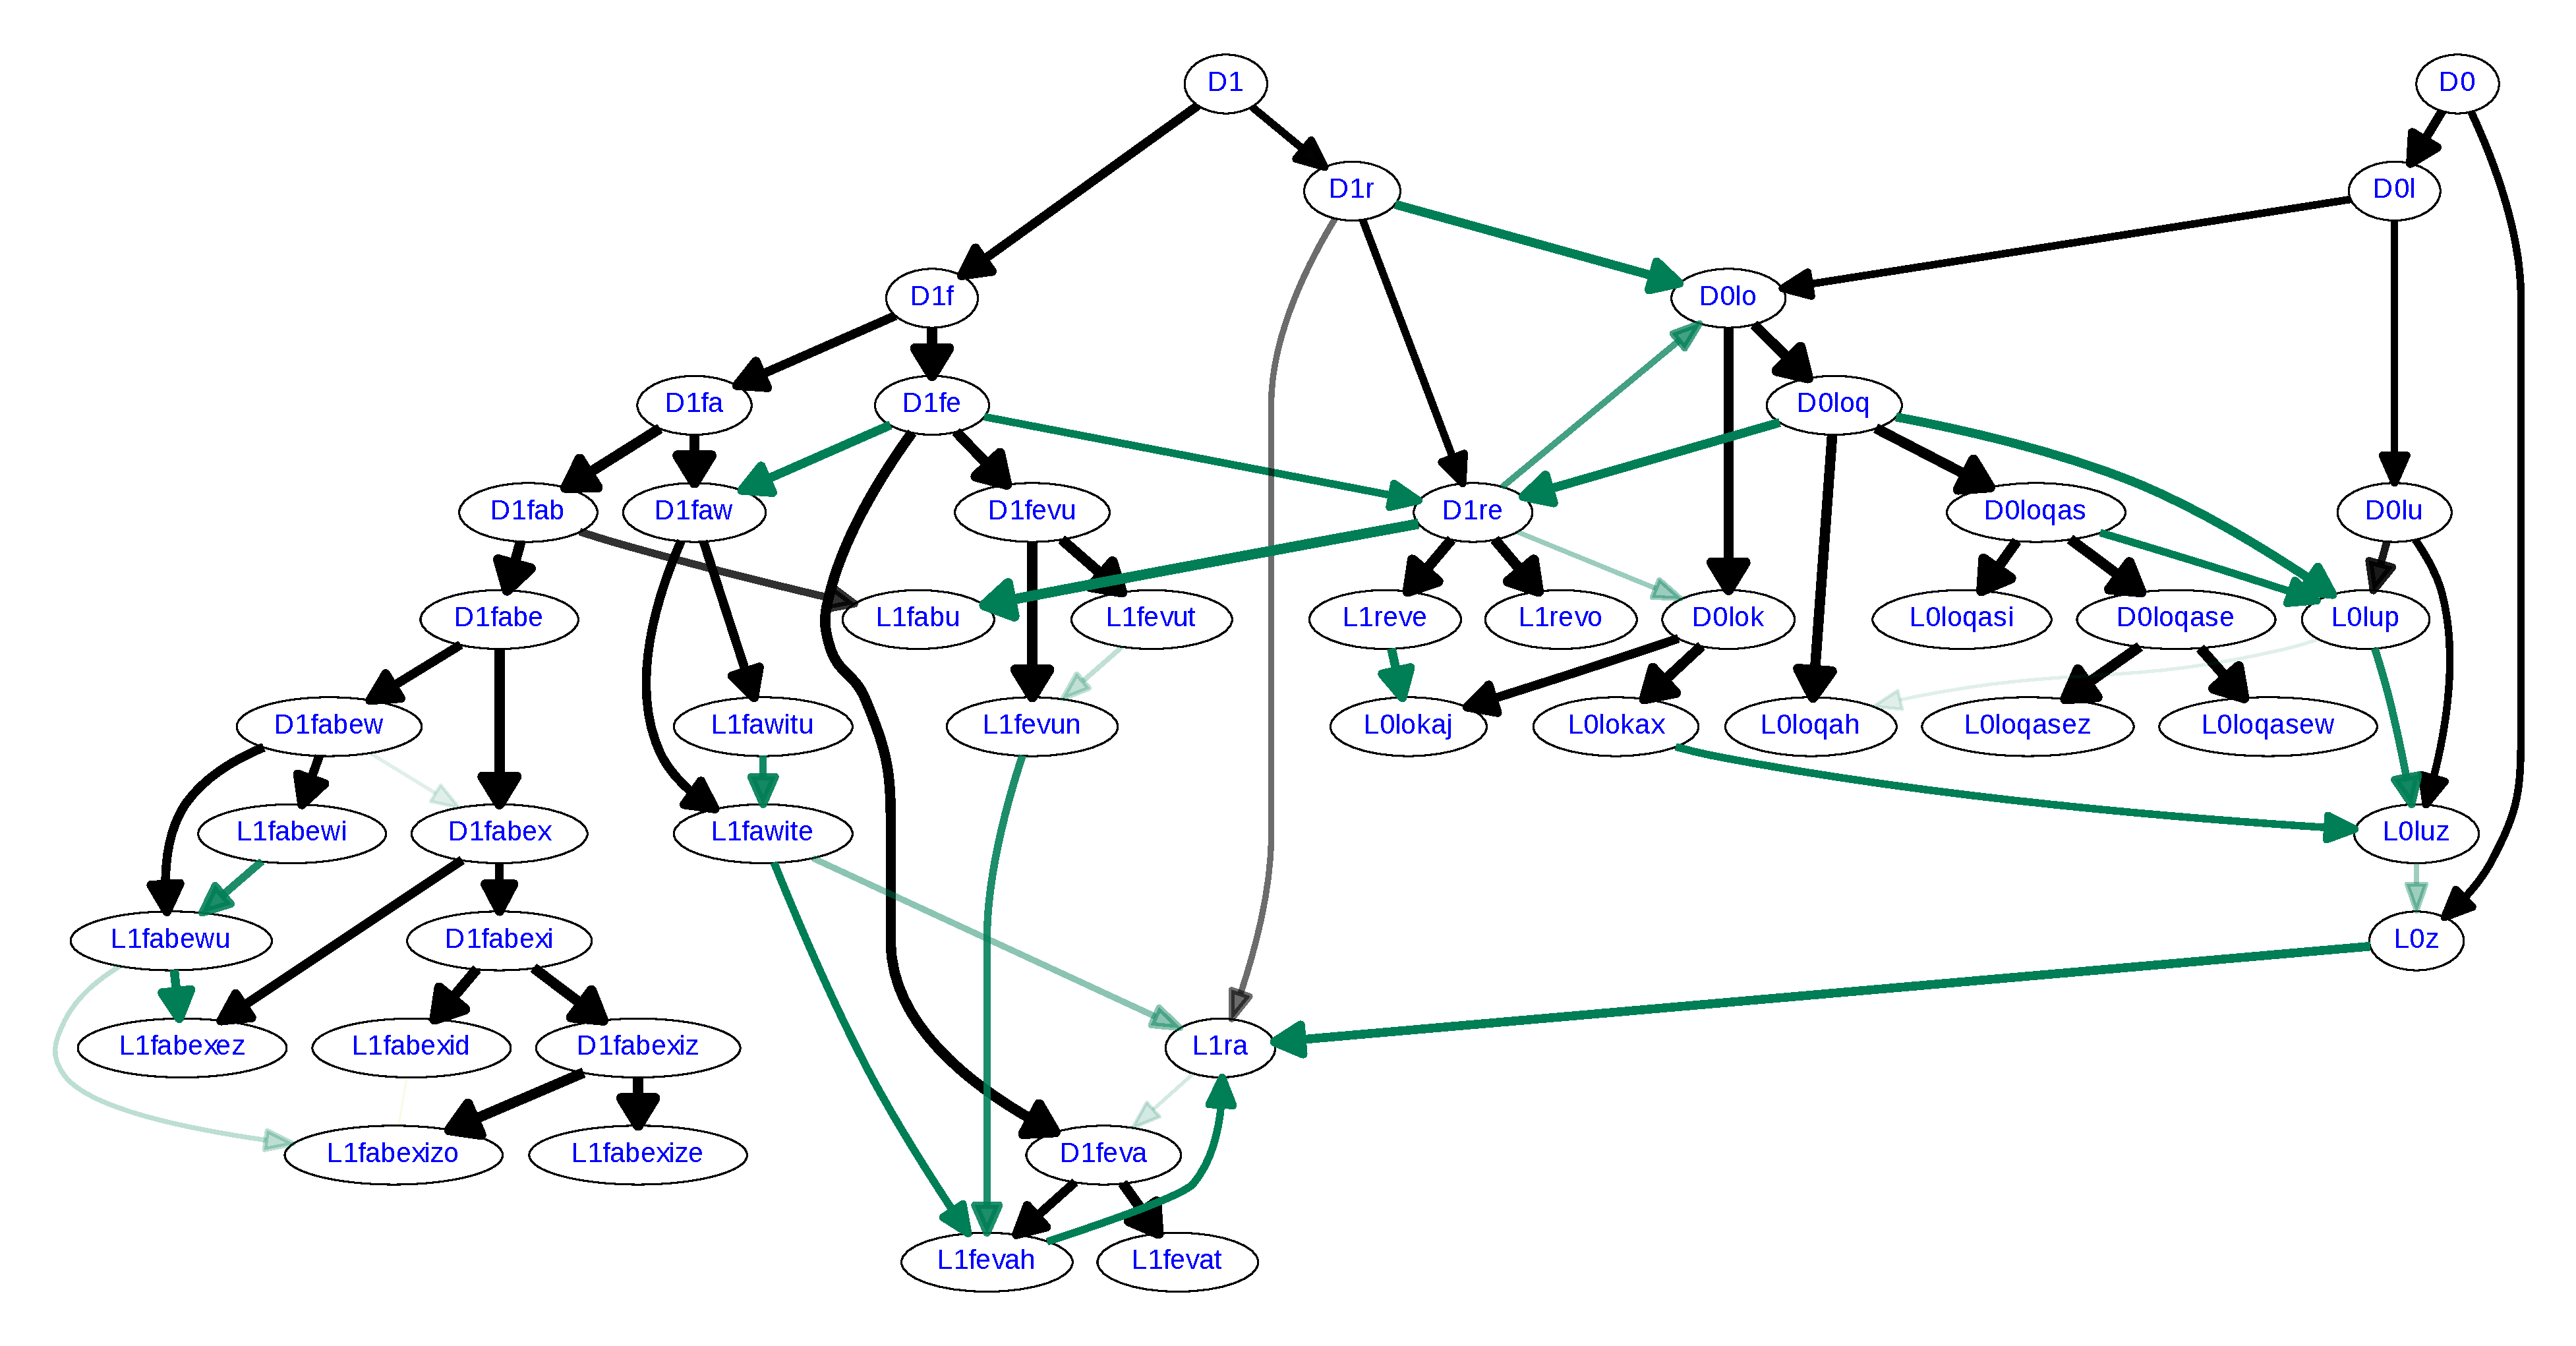
\includegraphics[width=\textwidth]{figures/sim-example-goldstandard-graph.pdf}
 \caption{An example of a simulated scenario, with complex interactions}
 \label{simulated-tree}
 \end{center}
\end{figure}

To showcase the geographic model, the maps in Figure \ref{simulated-maps} shows the final positions of each language for the same scenario, as well as the state of the simulation after 1,800 and 3,400 simulated years (i.e.\ 3,200 and 1,600 years before the final state). The three maps give an impression of how the initial population splits to fill the available space, and what type of contact is simulated by the model. Open contact channels are visualized in dark green (monodirectional contact) and light green (bidirectional, i.e.\ contact channels in both directions are open). The thickness of these lines represents the intensity of the contact, i.e.\ the rate at which lexical material is transmitted across each channel.

As in the cognate overlap maps used to visualize the shape of the inference problems in Chapter 4, the thickness of the black lines visualizes the strength of cognate overlaps between living languages at the respective point in time. In the comparison between the three stages, it becomes very obvious how some lines which were still strong thousands of years ago have faded into the background, reflecting the loss of similarity caused by lexical replacement.

\begin{sidewaysfigure}
\begin{subfigure}{0.25\hsize}
 \centering
 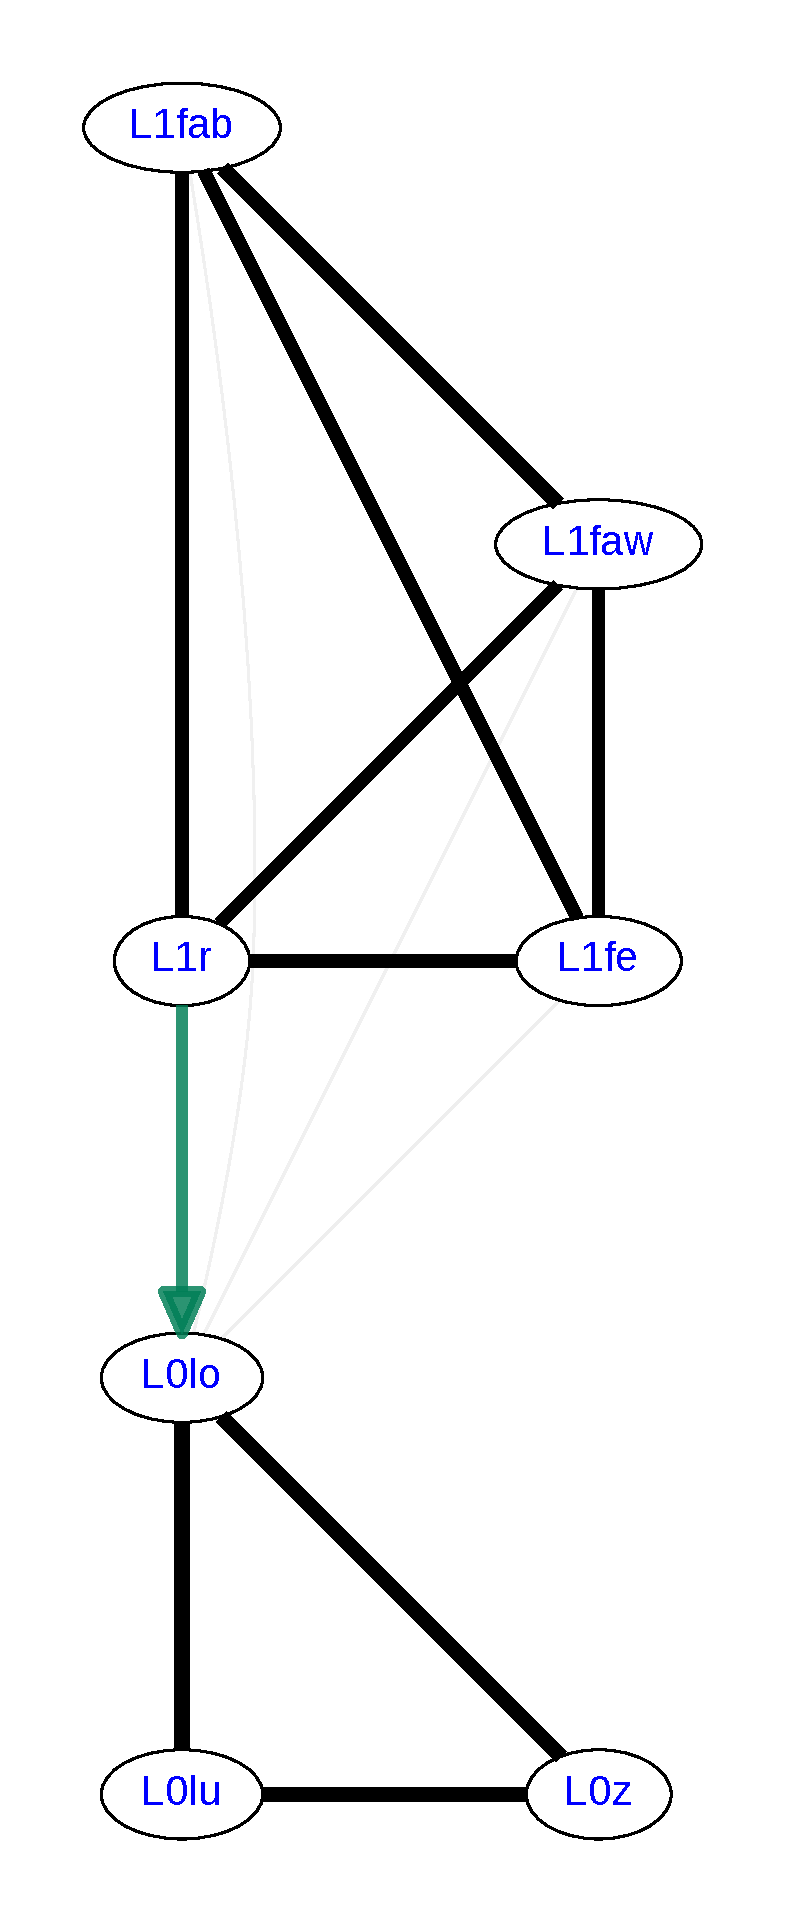
\includegraphics[scale=0.15]{figures/sim-example-initial-map.pdf}
 \caption{Situation after 1,800 simulated years.}
 \label{simulated-map-past}
\end{subfigure}
%
\begin{subfigure}{0.25\hsize}
 \centering
 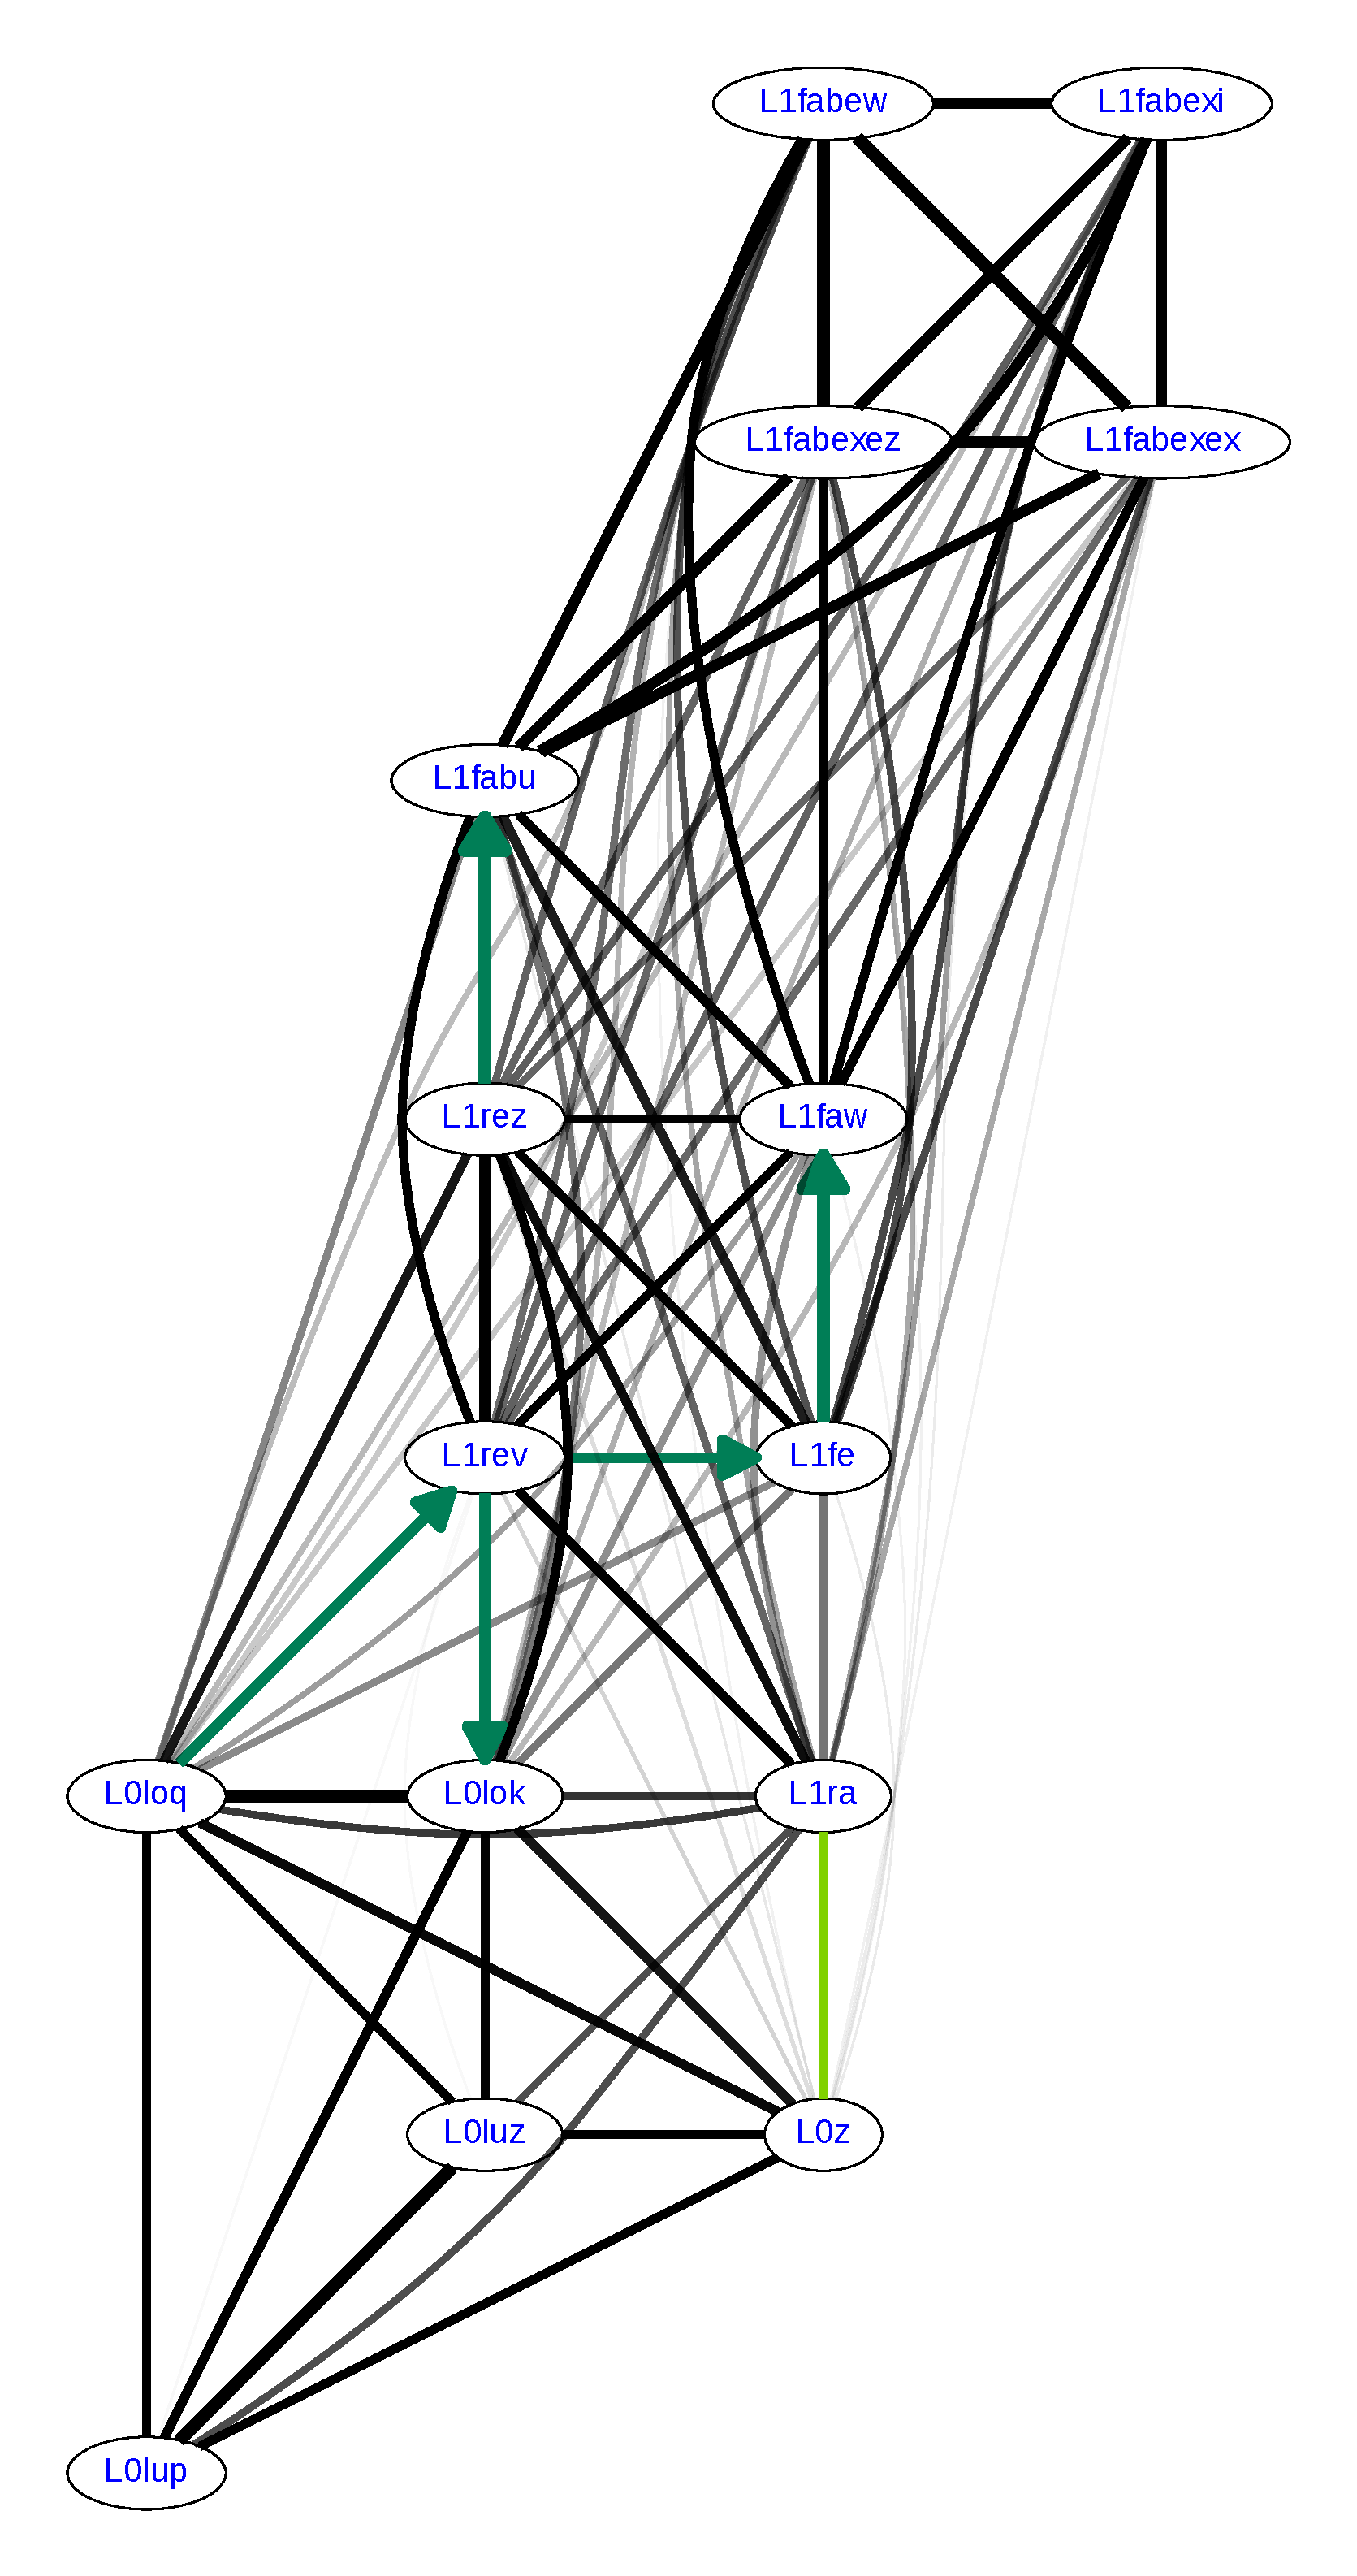
\includegraphics[scale=0.15]{figures/sim-example-past-map.pdf}
 \caption{Situation after 3,400 simulated years.}
 \label{simulated-map-past}
\end{subfigure}
%
\begin{subfigure}{0.4\hsize}
 \centering
 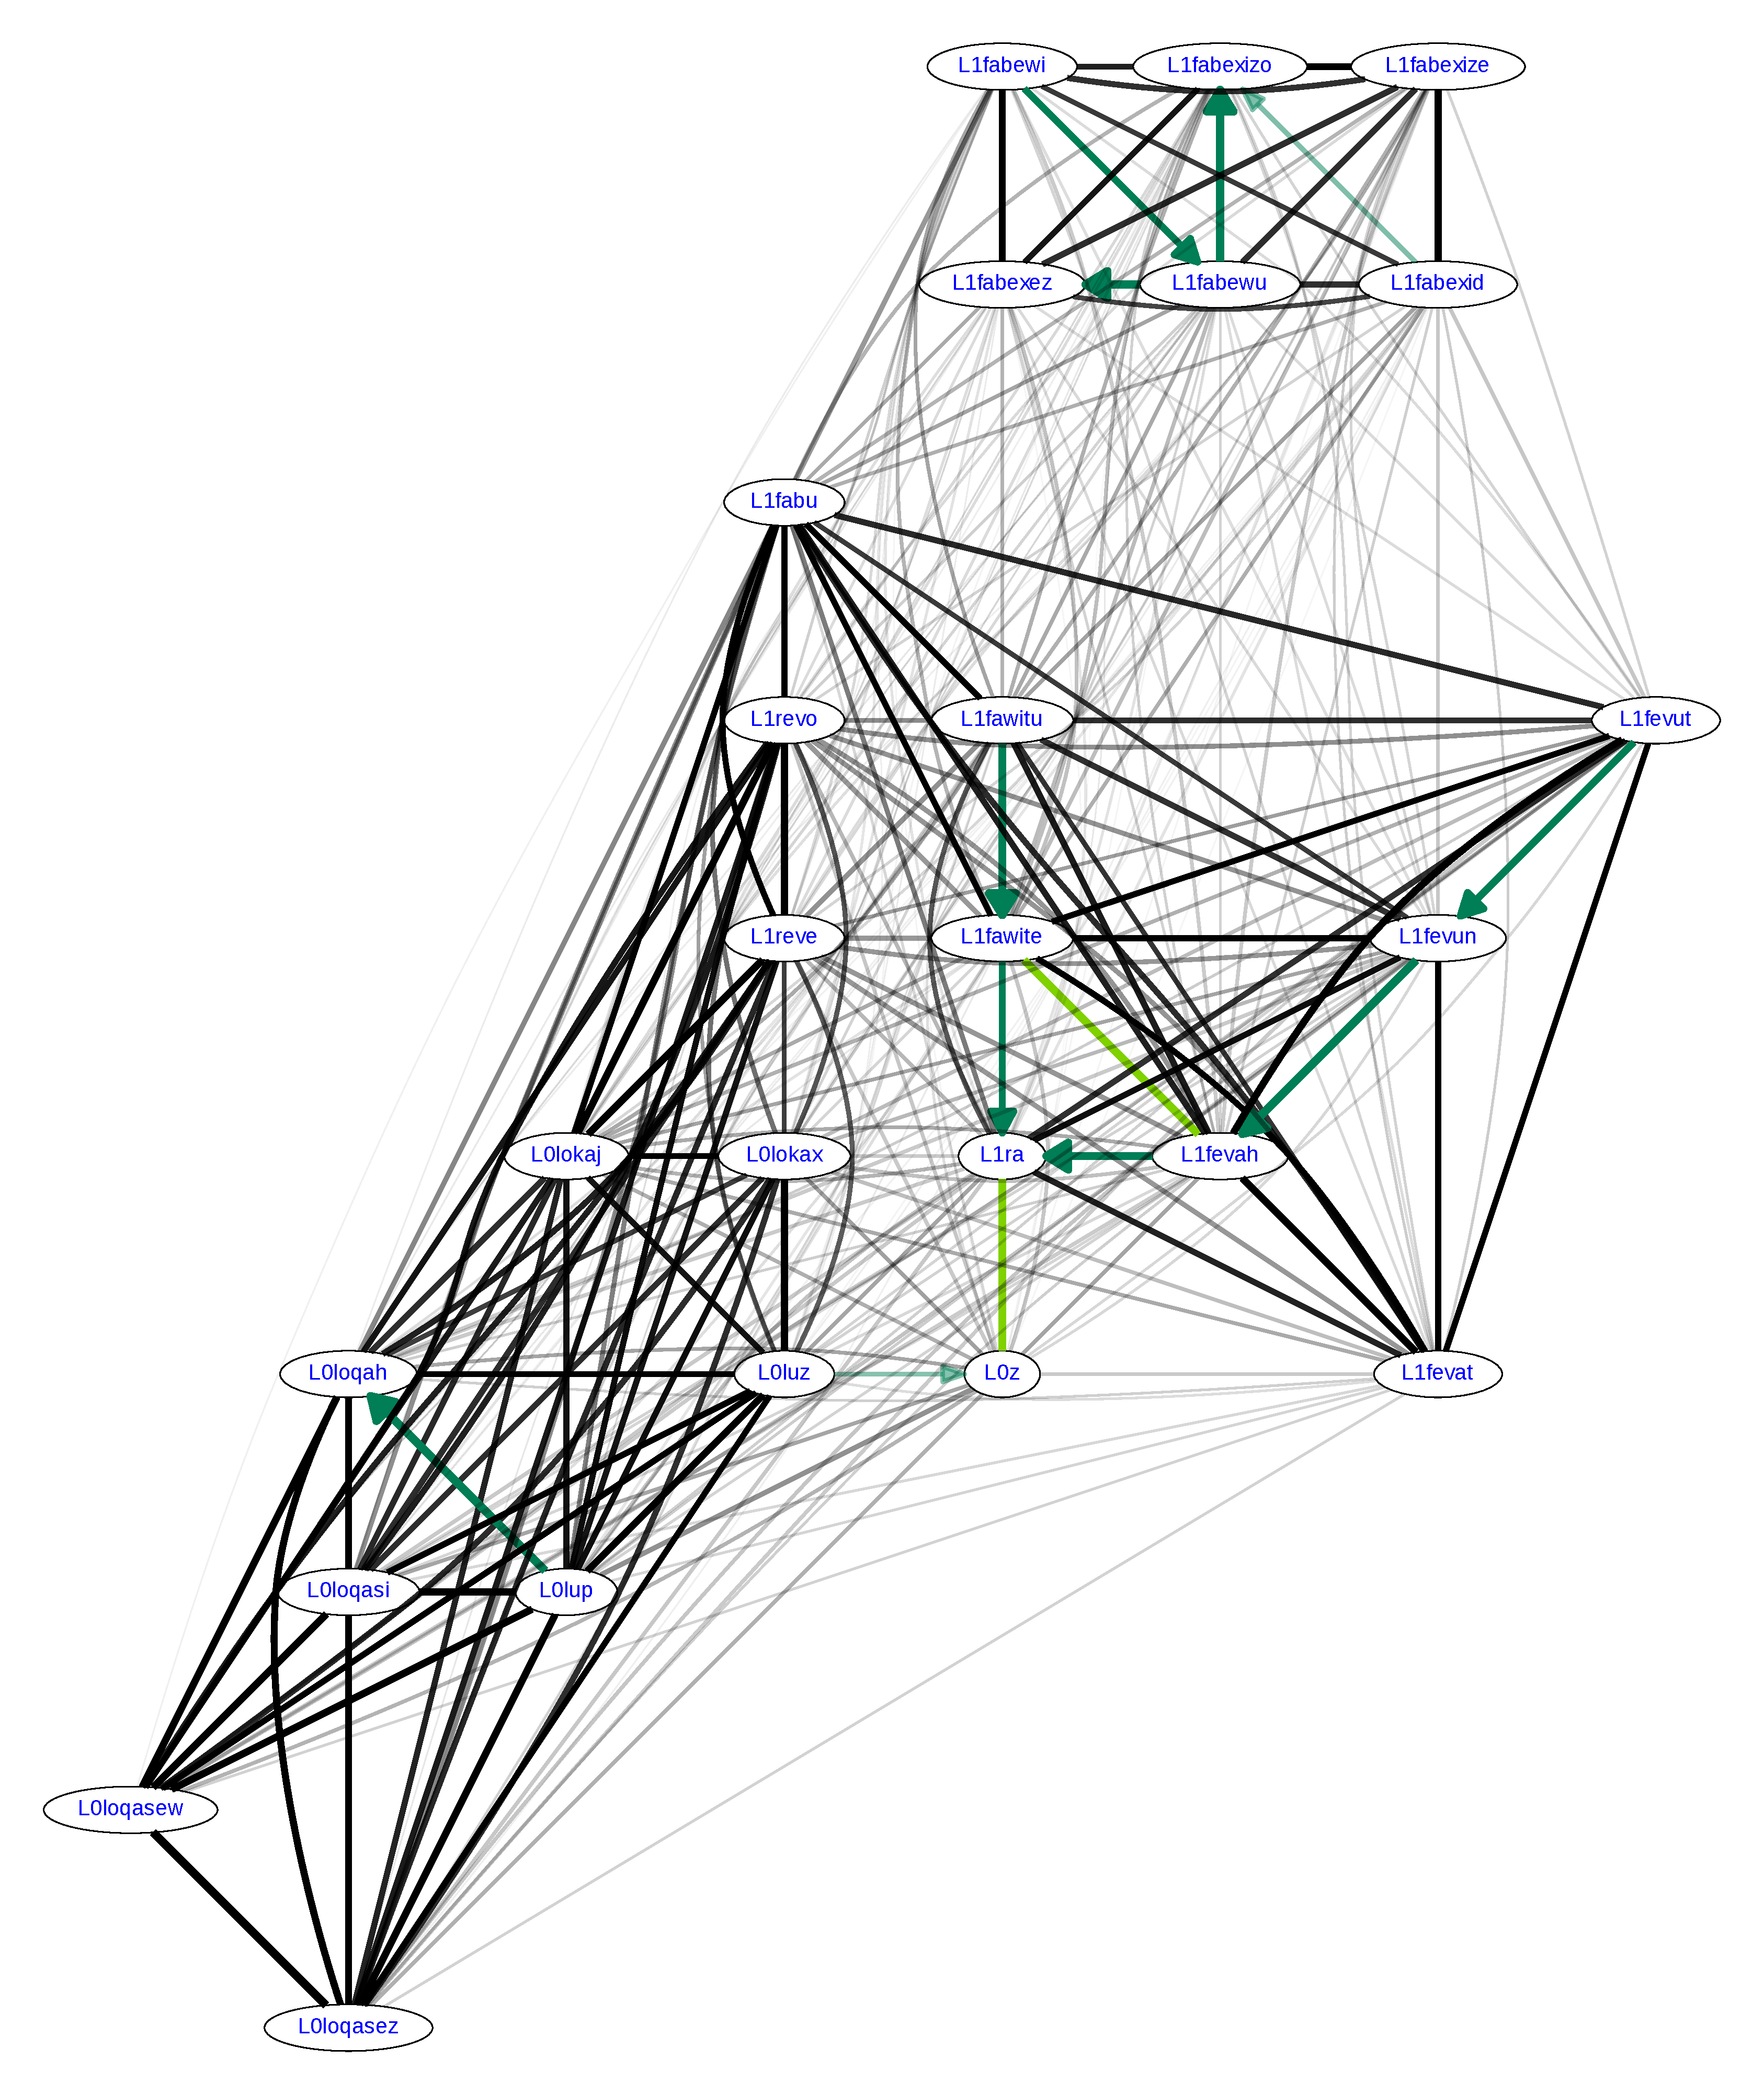
\includegraphics[scale=0.15]{figures/sim-example-present-map.pdf}
 \caption{Final situation after 5,000 simulated years.}
 \label{simulated-map-present}
\end{subfigure}
 \caption{Maps visualizing the situation of the example scenario at three points in time}
 \label{simulated-maps}
\end{sidewaysfigure}

To generate the evaluation set, a total of 50 scenarios were generated by simulation. Taken together, the simulated data contain 2,139 living languages distributed over 297 language families. In addition, a total of 7,128 intermediate (proto-)languages was modeled while producing the data for the living languages. In total, while generating the history of the languages, a total of 2,250,891 borrowing events were generated and logged, of which 380,571 events (16.9\%) turn up in the stored etymologies of one of the 2,139,000 lexical items in living languages.

In order to decide in which respects the simulation model does make sense (or not), the next section addresses the question whether the simulated data are similar enough to the NorthEuraLex data to be able to serve as additional test cases for validating my results. The section thereafter will answer the question whether the generated histories are non-trivial enough to provide some challenge to phylogenetic and lexical flow inference methods, and also varied enough to cover a wide array of situations we would expect to be faced with in actual linguistic histories.

\subsection{Are the scenarios realistic?}
The most trivial question to ask about the realism of the simulated histories is whether the distribution of cognate class sizes is similar enough to the one inferred from the NorthEuraLex data. The average size of cognate sets in the NorthEuraLex data is 2.253, whereas the simulation produces scenarios with average cognate sizes $2.164 \pm 0.192$, with the maximum being $2.656$, and the minimum $1.801$. This shows that the simulated cognate sets are similar in the size to the ones inferred by NorthEuraLex, indicating that the types of overlaps and therefore the information geometry will behave similarly. But since the average size of cognate sets heavily depends on the number of languages in the dataset, it might be more relevant to compare the average number of cognate sets per concept per language, and compare this measure across scenarios. In the simulated data, this number varies around $0.577 \pm 0.095$, with the minimum at $0.388$ and the maximum at $0.800$. The equivalent measure computed from the 
inferred correlate sets in NorthEuraLex is $0.497$, again fitting very well into the distribution of simulated scenarios. Finally, Figure \ref{cognate-class-sizes} shows the distribution of cognate class sizes in the simulated data next to the one for the classes automatically inferred from NorthEuraLex. It is clearly visible that both distributions are very similar, except for a much higher ratio of two-element cognate classes resulting from automated cognate detection. This fits well with the observations made when inspecting the inferred classes for \textsc{fish}, and is very likely an artefact of UPGMA clustering, which is sensitive to spurious pairwise similarities between elements which should form singleton classes. This difference also becomes visible when fitting Pareto distributions to the observed counts. The maximum likelihood estimates of the alpha parameter are $\alpha = 0.284$ for the NorthEuraLex data, but only $\alpha = 0.189$ for the simulated data. 

\begin{figure}
 \begin{center}
 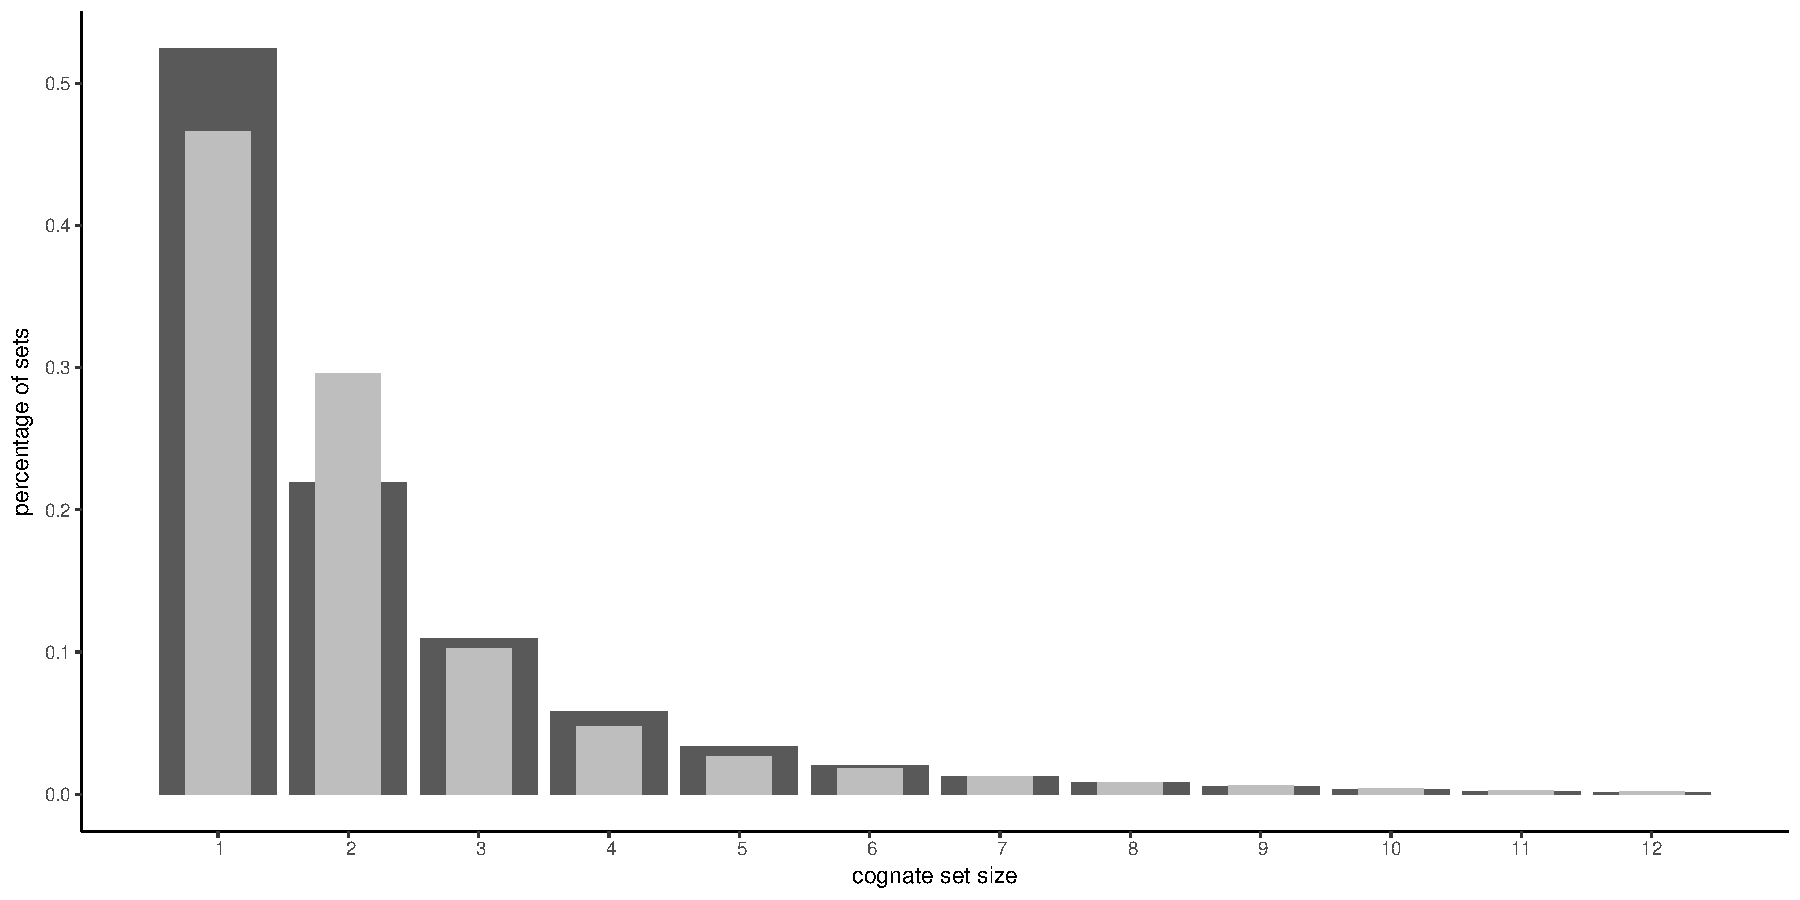
\includegraphics[width=\textwidth]{figures/cognate-set-sizes.pdf}
 \caption{Distributions of cognate class sizes on NorthEuraLex (gray) and simulated data (black)}
 \label{cognate-class-sizes}
 \end{center}
\end{figure}

To get a first impression of how realistic the amount of contact in the simulated data is, we can compute the percentage of words in the final data which were borrowed at some point in their history. Across all scenarios, 23.92\% of all attested words have at least one borrowing event as part of their history. Between scenarios, the ratio varied between 1.27\% and 38.53\%, with the mean at $23.07 \pm 8.71\%$. This is very much in line with the numbers derived from the WOLD database and summarized in \cite{tadmor2009}, where the ratio of loans in content words varied between 1.3\% (\ili{Mandarin Chinese}) and 65.6\% (Selice \ili{Romani}), and the average ratio of loans across all languages was $24.2\%$. Therefore, both the overall frequency of loans and the variance of the ratio across simulated languages and scenarios are very realistic.

With respect to lexical replacement, we can compute the distribution of word ages from the logged histories. For each word in a living language, we can trace back the history to the point where the word came into existence as a word for the concept in question by a replacement event (a mutation, in biological terms), or back all the way to one of the initial languages. Across all scenarios, 16.93\% of the words could be traced back to one of the initial languages. Unsurprisingly, the distribution almost exactly fits an exponential curve with our loss rate of about 0.036\% per year, leading to e.g.\ 3.42\% of words older than 4,500 years, 6.83\% between 2,000 and 2,500 years old, and 16.29\% younger than 500 years. The language-wide averages of word ages were distributed around $2357.43 \pm 133.84$. I have found it impossible to find even rough cross-linguistic estimates for the word age distribution across entire lexica of modern languages. Still, we can use some etymological resources to get a first 
impression whether the numbers seem realistic. \cite{sammallahti1988} provides the most up-to-date overview of the known lexicon of Proto-Uralic\il{Uralic languages} as well as some later proto-languages of branches such as Finno-Ugric\il{Finno-Ugric languages}. He counts 124 Uralic stems as being reconstructable for Proto-Uralic (perhaps 7,000 years ago), about 290 additional ones for Proto-Finno-Ugric (5,000 years ago), and 150 more for Proto-Finno-Permic\il{Finno-Permic languages} (a contested subgrouping of perhaps 4,000 years). \cite{janhunen1977} reconstructs about 700 stems in total for Proto-Samoyedic\il{Samoyedic languages}, at about 2,500 years of age. A typical dictionary of a fully known language that is sorted by lexical roots, such as \cite{de_vaan_2008} for \ili{Latin} or \cite{lehtisalo_1956} for \ili{Nenets}, covers the history of about 2,000 roots. We can thus assume that this is roughly the number of etyma which we can assume for an unwritten language. Fitting an exponential curve to these 
five data-points, our replacement rate of 0.036\% per year, or about 30.24\% per millennium, fits almost perfectly. Calculating the distribution of word ages across this curve (and counting every word older than PFU as 5,000 years old in the same way as I need to do it for the simulated data), we arrive at a mean age of $2317.5$ years, which again fits very well into the distribution of values derived from the simulated data. The distorting effect of borrowings on reconstructability therefore seems to have a very negligible influence.

Another interesting question to ask about the distribution of word ages is whether there are conservative languages which tend to conserve more ancient words across the basic lexicon, whether due to limited lexical contact, or an inherent tendency to slower lexical replacement. This is equivalent to the question whether different languages can have vastly different average replacement rates across a timescale of thousands of years. While there is considerable evidence that replacement rates can vary a lot on the short term \citep{atkinson_ea_2008}, it is unclear whether these differences are random fluctuations which might equal out with time, or whether they are inherent properties of language systems which remain in place for millennia. On the simulated data, while the underlying model of divergence operates at a global replacement rate for all languages, replacement by borrowing leads to very different retention rates. In the most conservative simulated language, the average word age was $3475.92$, as 
opposed to $1892.89$ in the language with the least stable vocabulary. This shows that a mixture of a variance in global replacement rate for each scenario already leads to an interesting and realistic range of measurable conservativity in the simulated languages.

The next relevant point of comparison is the shape of the trees. An essential observable property of binary trees is their balancedness, which can be defined in many different ways, each capturing a different type of asymmetric behavior. \cite{holman2005} analyzes linguistic trees in this framework, making the very interesting observation that language trees have different structure than would be generated by simple birth and death processes, even if we allow different diversification rates for each branch. Holman uses the weighted imbalance score by \cite{purvis_ea_2002}, to show that actual language trees are much more unbalanced than such a model would predict. The imbalance score for a binary node $l$ with children $l_1$ and $l_2$ is computed as $I(l) := \frac{B - \lceil S/2 \rceil}{S - \lceil S/2 \rceil - 1}$, where $S$ is the number of nodes on the subtree under $l$, and $B$ is the maximum of the sizes of the two subtrees under $l_1$ and $l_2$. $I(l)$ will be 0 for a maximally balanced node (in the 
sense that a node with this number of descendants could not be more balanced), and close to 1.0 if one of the children is a leaf and many other nodes are descendants of the other child. For an entire tree, the \isi{weighted imbalance score} is a weighted mean over these node-based scores, where the weight $w(l)$ is $1$ if S is odd, $w = (S-1)/S$ if S is even and I > 0, and $w = 2(S-1)/S$ if S is even and $I = 0$ (such that completely balanced nodes count twice). This score is defined in such a way that the expected value for trees generated by a birth and death process is 0.5. As Holman shows, the weighted imbalance scores for actual language trees are significantly higher than that, clustering around 0.7. The simulated trees have weighted imbalance scores between $0.587$ and $0.820$, with the mean at $0.698 \pm 0.053$, which fits Holman's results surprisingly well. It seems that a simple death-by-replacement model on a constrained geography is all that is needed to explain the imbalance in empirically 
observed trees, without any need to allow for branch-specific diversification rates or similar devices.

There are some additional phenomena which are so commonly observed in historical linguistics that realistic datasets should contain some instances of them. One of these are isolates\is{isolate}, which can here simply be defined as phyla with only one surviving descendant language. According to the Glottolog classification, roughly half of the world's families are isolates, and this is also roughly the ratio of isolates in NorthEuraLex (9 out of 21 families). While isolates are not interesting for evaluating phylogenetic methods, they can still be involved in some interesting contact scenarios, and should therefore be present at least in a few scenarios. So does the simulation model, where isolates can only occur if one of the initial languages never splits during 5,000 simulated years, or if all but one of the potentially many languages from a family are replaced by neighboring families branching and expanding into its territory, produce a significant number of isolates? Across all scenarios, only 16 of the 
270 families generated by the simulation model are isolates, a number which is unrealistically low compared to the large numbers of isolates we observe in many regions of the world. While this is not a problem for evaluation purposes (as long as some isolates are present), it might still be worthwhile to speculate why so many more isolates occur in reality. One possible explanation is that the over-simplified geography (without remote mountain valleys) does not generate enough niches for smaller families to survive. Moreover, the constraint of having exactly one language per place will counteract the arising of true isolates. In reality, if two villages with closely related dialects of an isolate are surrounded by completely unrelated languages, the two villages might prefer close contacts among each other, counteracting the divergence into separate languages.

As a final point, a problem of realistic complexity should contain substrates. To recapitulate, a substrate relationship is one possible result of language shift, when the speakers of one language rapidly shift to another language, but the shift is incomplete in leaving traces of the ancestral language (a substrate) in the new language. In historical linguistics, the term \textit{\isi{substrate language}} is often used in the sense of an otherwise unattested language whose existence can only be reconstructed from a layer of words which have no etymology in the respective family. With access to the simulated history of each word in a large datastructure, it becomes possible to compute the ratio of words which were borrowed at some point from a substrate language, and the number of languages without living descendants which became sources of such borrowings. Analyzing the histories of all words in the simulated dataset, we find that 5.04\% of all words have a substrate history by our definition. Averaging 
across scenarios, $65.16 \pm 37.05$ languages, i.e.\ slightly less than half of the $142.56 \pm 62.66$ extinct languages, played the role of a substrate language during the history of at least one word. Of $78.62 \pm 37.41$ contacts, $26.14 \pm 17.24$ occur with a donor language which leaves no living descendant in an average scenario. It is difficult to assess how realistic these numbers are, because in the real world, words without an etymology are often difficult to attribute to one common substrate donor. Still, there tend to be many instances of unknown substrates even in the history of a very limited linguistic region such as Northern Europe. The most famous instance is an unknown substrate in Germanic\il{Germanic languages} consisting of mainly maritime vocabulary such as \textit{*strand\={o}} `beach' and \textit{*seglan} `sail'. Originally assumed to comprise a third of the common Germanic lexicon, it has been shrinking in size as additional Indo-European etymologies for Germanic lexemes are being 
established. While some scholars like \cite{hawkins1990} continue to advocate it, it now seems to be on the way to becoming a minority position. Less contested instances of substrates in the North are a layer of pre-Uralic lexical material in the \ili{Saami languages} \citep{aikio2004}, and a different pre-Uralic substrate which heavily influenced the \ili{Samoyedic languages} \citep[e.g.][]{helimski1998}. Given the ubiquity of such examples even in an area with a rather short post-glacial settlement history, it makes sense to have substrate relationships occur so frequently in the simulated data.

\subsection{Are the scenarios interesting?}
The second question about the adequacy of the simulation model is whether the simulated scenarios are difficult and varied enough to make the results of evaluation interesting. To answer the first question, this section analyzes how well the tree signal is recoverable from the overlap of cognate classes alone, and, answering the same question from a slightly different angle, how well the cognate class boundaries coincide with phylogenetic units. Then, the identifiability of contact events is analyzed in order to quantify the maximum performance that we could hope an ideal system to achieve on the lexical flow inference task. For an answer to the second question, the section goes through some phenomena that we might expect to occur in actual linguistic histories of geographical areas where several language families are neighbors for several millennia, and discusses to what extent these phenomena also occur in the simulated data.

A very direct way of assessing the difficulty of phylogeny inference is to measure the recoverability of the tree signal from the cognate data. If the cognate overlaps perfectly encode the tree structure, we should have $|c(A,B)|$ > $|c(A,C)|$, $|c(B,C)|$ in all configurations where $A$ and $B$ are more closely related than either is with $C$, or more precisely, if the lowest common ancestor of $A$ and $B$ is a descendant of the lowest common ancestors of $A$ and $C$ as well as $B$ and $C$. In the simulated scenarios, the cognate overlaps match the criterion for $89.32 \pm 6.87\%$ of such triples. On the automatically inferred cognates derived from NorthEuraLex and the reduced Glottolog tree, the value is $82.28\%$, i.e.\ comparable in complexity to the more difficult simulated scenarios. In the most difficult scenario, the inequality only holds for $64.91\%$ of triples, and the easiest scenario (with only one contact in 5,000 years) has $100\%$. Given the presence of errors in automated cognate judgments, it is hardly surprising that the NorthEuraLex task is on the more difficult end of the scale.

A more strict measure of the difficulty of the inference task is the fit of cognate set boundaries to phylogenetic units. More precisely, we are interested in the percentage of cognate sets which exactly correspond to the descendants of a single phylogenetic node. Note that this correspondence is not only destroyed by borrowing, but also by lexical replacement in one language of the unit, though the latter situation will produce a new cognate set which is aligned to a phylogenetic unit of trivial size. On the simulated scenarios, the distribution of this percentage can be summarized as $17.33 \pm 4.98\%$. The value of $10.06\%$ on NorthEuraLex cognates and the Glottolog tree is close enough to this distribution to provide additional evidence that the simulated scenarios are quite realistic in difficulty. However, the NorthEuraLex data are by this measure more challenging even than the worst of 50 simulated scenarios at $10.28\%$. This is again easily explainable by the existence of erroneous automated 
cognacy judgments, as both false positives and false negatives will destroy perfect alignments of cognate classes with phylogenetic units. On the tree signal, the errors apparently almost cancel out, not detracting much from recoverability, whereas the matches of entire cognate sets are much more sensitive to uncertain cognacy judgments. This has problematic implications for algorithms building on cognate set overlaps, such as the lexical flow inference procedure I will be exploring.

An important question to ask about the data concerns the identifiability of contact events. How many of the contact channels still have visible consequences in the living languages, in the sense that they are part of the histories of enough words in living languages to go beyond the detection threshold of 20 loans? This measure gives us an upper bound on the performance we could hope to achieve with any algorithm which reconstructs previous reflexes of cognate sets and then tries to infer contact events. In the simulated data, 67.6\% of all simulated contacts were still visible by this definition, resulting in an average of $49.68 \pm 23.16$ detectable contacts per scenario. This number implies that certainly enough interesting contact patterns occur in the simulated data, and the consequences of two thirds of these are still in principle detectable in the output data.

Finally, a few words can be said about the variability of patterns encountered in the simulated data. Using graph terminology, there are 27,164 unshielded triples in the gold standard flow graphs. 15.05\% of these are colliders, where a single language is influenced by two different languages. 550 (13.45\%) of these colliders connect languages which have not interacted in any way before. As we will see in the next chapter, this type of collider is easily detectable using v-structure tests, giving us very reliable directionality information. The problem is that out of 12,179 lateral connections whose directionality we will want to determine, only 870 take part in such strict colliders, and 4,088 lateral connections are part of any type of collider. This means that we only have completely reliable directionality information for 7.14\% of these connections, and some direct evidence for 33.6\%. The directionality of two thirds of our lateral links would thus have to be determined by some form of constraint 
propagation, which will cause some problems if our unshielded collider tests are not completely reliable. To sum up, the simulated instances are definitely challenging enough to provide useful information about the potential of causal inference for lexical flow inference.

Coming to phenomena of more immediate linguistic interest, we first consider chains of loans, where lexical material is transmitted from one language to another through a third language which serves as a bridge, whereas the first two languages are not directly in contact. Such chains would mirror the phenomenon of wanderw\"orter such as \textit{sugar} or \textit{wine}, which were not borrowed from one original language into every language which now uses them, but travelled from language to language together with the trade goods, reaching remote geographical areas via trading intermediates. In the simulated data, 16.4\% of words with a borrowing history were borrowed twice, and 2.9\% were borrowed three or more times. There is thus a fair amount of wanderwort-like word histories in the data, adding to the realism of the simulated scenarios.

Another phenomenon whose frequency is worthwhile to investigate is \isi{internal borrowing} within the same language family, i.e. the situation in which a word can be replaced by a cognate word. In the simulated data, because related languages are more likely to be neighbors, internal borrowing happens quite often, so that in $26.280\%$ of all generated borrowing events one cognate set was replaced by the same set, not changing anything about the data. Across scenarios, this percentage was pretty stable at $29.531 \pm 5.80\%$, although there are some outliers with the maximum at $67.3\%$. Set-internal borrowings are obviously a problem for contact detection algorithms which work on the level of cognate sets, because such borrowings do not leave any detectable traces.

\section{Potential further uses of simulated scenarios}
In addition to their usage as test cases for evaluating my methods, other researchers might want to use simulated scenarios as generated by my model as well. For instance, because each event during the simulation is logged in a format which allows the complete history of each word to be tracked explicitly, it becomes possible to evaluate loanword detection algorithms on much larger datasets than the real datasets which are currently and will ever be available.

This also applies to the comparative evaluation of methods and algorithms for tasks wich are closely related to lexical flow inference, such as the inference of different types of phylogenetic networks. In this context, the simulation could be used to assess the impact of lateral transfer on the reliability of phylogenetic inference methods, e.g.\ for practical experiments reinforcing the empirical findings by \cite{greenhill_ea_2009} or the mathematical results of \cite{roch_snir_2012}, both indicating that phylogenetic inference is quite robust to realistic amounts of lateral transfer.

For all these purposes, the simulated scenarios are distributed together with this book in various standard formats (trees in Newick format, cognacy data in a Nexus format readable by the most common software tools in phylogenetic inference). Moreover, my Java programs for generating more scenarios of this type, as well as the parsers for the log files which are necessary to extract statistical information of the type I was covering in this chapter, will be packaged and released as standalone executables along with their source code in order to allow other researchers to adapt the simulation model to their requirements, or experiment with different parameter settings than the ones I have been operating on here.
